\section{General (Victor pour descriptions globale)}
\subsection{Objectifs généraux de la catégorie du challenge}
% Contenu à rédiger ici

\subsection{Encoding (Encoding challenge)}
Cette première sous-partie de la catégorie General aborde les différentes
méthodes de représentation de l'information, essentielles au transport et
à l'échange de données. La maîtrise des conversions entre des formats
comme le binaire, l'hexadécimal ou le Base64 constitue un prérequis
indispensable pour aborder des défis cryptographiques plus complexes. Il
est fondamental de bien distinguer l'encodage du chiffrement : le premier
est une transformation de format, publique et réversible, qui ne vise pas
à garantir la confidentialité, contrairement au second.

Nous avons décidé de présenter le dernier challenge de cette partie, nommé
\textit{Encoding challenge}.

\subsubsection{Objectifs}
L'objectif de ce challenge consiste à développer un script pour automatiser
l'interaction avec un serveur distant de CryptoHack. Le processus implique
la réception de données encodées selon diverses méthodes (Base64,
hexadécimal, ROT13, BigInt, et UTF-8), leur décodage approprié, puis le
renvoi de la valeur décodée au serveur.

Pour valider le challenge et obtenir le flag, il est impératif d'exécuter
cette séquence de réception, décodage et renvoi avec succès cent fois
consécutives. Cette contrainte requiert une solution entièrement
automatisée, capable de gérer dynamiquement les différents types
d'encodage rencontrés.

\subsubsection{Méthode}
Le challenge met à disposition un script partiel qui présente la manière
d'envoyer et recevoir des données avec le serveur, ainsi que le script
exécuté côté serveur pour vérifier les valeurs qui lui ont été transmises.
Ces scripts nous ont permis de comprendre le format des données transmises.

La communication avec le serveur s'effectue via l'échange d'objets au format
JSON. Pour chaque itération du challenge, le serveur envoie une requête
structurée de la manière suivante~:

\begin{verbatim}
{
    "type": "type_d_encodage",
    "encoded": "donnees_encodees"
}
\end{verbatim}

Notre script doit alors analyser cette requête, appliquer la méthode de
décodage appropriée, et renvoyer la solution au serveur sous le format JSON
attendu~:

\begin{verbatim}
{
    "decoded": "donnees_decodees"
}
\end{verbatim}

Le script côté serveur vérifie alors la validité des données décodées, puis
si cela est valide, crée un nouveau challenge. Si notre script résout cent
challenges, la prochaine requête au serveur permettra d'afficher le
\textit{flag} dans la sortie standard.

\subsubsection{Résultat}
Pour résoudre le challenge, nous nous sommes donc appuyés sur les scripts
python du challenge afin de développer un script de résolution (voir ...).

\begin{figure}[H]
    \centering
    % La commande pour insérer l'image.
    % 'width=0.8\linewidth' signifie que l'image fera 80% de la largeur du
    % texte.
    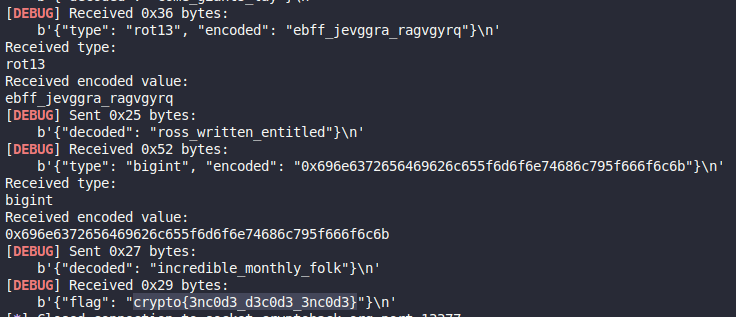
\includegraphics[width=0.8\linewidth]{Images/Encode/encode_chall_result.png}

    % La légende qui apparaîtra sous l'image.
    \caption{Ceci est le schéma explicatif de notre méthode.}

    % L'étiquette pour y faire référence plus tard.
    \label{fig:encodeChallRes}
\end{figure}

Après cent requêtes valides, le \textit{flag}
\textit{crypto\{3nc0d3\_d3c0d3\_3nc0d3\}} a été obtenu, permettant la
validation du challenge.

\subsection{Xor (Lemur)}
La deuxième sous-partie de la catégorie \textit{General} est consacrée à
l'opération XOR (ou exclusif), un concept fondamental en cryptographie
constituant l'une des briques de base de nombreux algorithmes de
chiffrement. Sa simplicité de mise en œuvre et ses propriétés mathématiques
uniques en font un outil puissant pour manipuler l'information.

Comprendre le fonctionnement du XOR est une étape cruciale, car il se situe
à la frontière entre l'opération logique et le chiffrement. L'une de ses
propriétés essentielles est sa réversibilité: appliquer deux fois la même
clé XOR à une donnée permet de retrouver la donnée originale
($A \oplus K \oplus K = A$). Cette caractéristique est au cœur de son
utilisation dans des chiffrements à flux comme le One-Time Pad.

Nous avons décidé de présenter le challenge le plus représentatif de cette
partie, nommé \textit{Lemur XOR}.

\subsubsection{Objectifs}
Le but de ce challenge est de retrouver le \textit{flag}, à partir de deux
images fournies : \texttt{lemur.png} et \texttt{flag.png}. L'énoncé nous
apprend que ces deux images ont été chiffrées avec l'opération XOR en
utilisant la même clé secrète.

\begin{figure}[htbp] % L'environnement figure global
    \centering % Pour centrer le bloc des deux images

    \begin{minipage}{0.48\textwidth}
        \centering
        
\includegraphics[width=\linewidth]{Images/Lemur/flag.png}
        % Première image
    \end{minipage}
    \hfill % Ajoute un espace horizontal flexible entre les images
    \begin{minipage}{0.48\textwidth}
        \centering
        
\includegraphics[width=\linewidth]{Images/Lemur/lemur.png}
        % Deuxième image
    \end{minipage}

    \caption{Ceci est la légende commune pour les deux images.}
    \label{fig:deux-images}
\end{figure}

Le principe de résolution repose sur le fait qu'appliquer deux fois un XOR
avec la même clé annule l'opération. En effectuant un XOR entre les deux
images chiffrées que nous possédons, la clé secrète commune s'élimine,
ne laissant que le résultat du XOR entre les deux images originales. C'est
sur cette image combinée que le \textit{flag} devrait devenir visible.

\subsubsection{Méthode}
Pour résoudre ce challenge, nous avons utilisé un script en Python avec la
bibliothèque de manipulation d'images \textbf{Pillow}. Nous avons commencé
par charger les deux images, \texttt{lemur.png} et \texttt{flag.png}.
Conformément aux instructions, nous avons appliqué l'opération XOR pixel
par pixel sur les valeurs de couleur RVB, et non sur les fichiers entiers.

Nous avons donc parcouru les deux images simultanément et calculé la nouvelle
valeur de chaque pixel en effectuant un XOR sur ses composantes rouge,
verte et bleue. Nous avons ensuite utilisé ces nouveaux pixels pour
construire une image de sortie de mêmes dimensions que nous avons sauvegardée.

\subsubsection{Résultat}
\begin{figure}[H]
    \centering
    % La commande pour insérer l'image.
    % 'width=0.8\linewidth' signifie que l'image fera 80% de la largeur du
    % texte.
    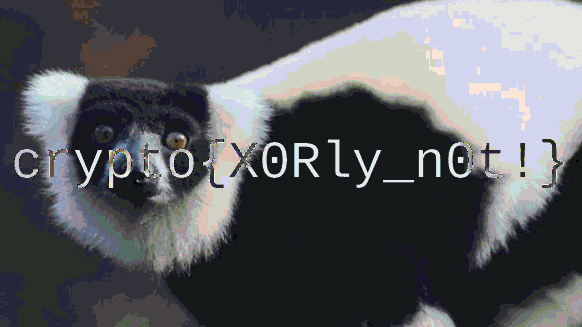
\includegraphics[width=0.8\linewidth]{Images/Lemur/xored_result.png}

    % La légende qui apparaîtra sous l'image.
    \caption{Ceci est le schéma explicatif de notre méthode.}

    % L'étiquette pour y faire référence plus tard.
    \label{fig:encodeChallRes}
\end{figure}

\subsection{Data formats (Transparency)}
\subsubsection{Introduction}
Le challenge s'appuie sur le principe de \emph{Certificate Transparency}
(CT), une mesure de sécurité imposée aux Autorités de Certification (CA)
pour garantir la transparence dans la délivrance des certificats TLS.

Un certificat TLS (souvent appelé certificat SSL ou certificat numérique)
est un document électronique qui remplit deux fonctions principales : il authentifie l'identité d'un site web ou d'un domaine auprès des clients (navigateurs, applications), et il permet d'établir une connexion chiffrée (TLS) entre le client et le serveur, garantissant la confidentialité et l'intégrité des données échangées.

Un \emph{CT log} est une base de données publique, append-only (où l'on ne
peut qu'ajouter des entrées) dans laquelle les certificats émis par les CA
sont enregistrés. Aujourd'hui, les principales CA doivent publier (ou
« soumettre ») chaque certificat qu'elles émettent dans au moins deux logs
CT publics pour qu'il soit accepté et reconnu comme valide par les
navigateurs modernes.

Ces logs sont audités et surveillés : chacun peut vérifier les entrées,
détecter des certificats inattendus, ou vérifier la cohérence de la
structure interne (par exemple via un arbre de Merkle) pour s'assurer
qu'on ne cache pas d'entrées.

\subsubsection{Objectifs}
L'objectif de ce challenge est double. Premièrement, il s'agit de retrouver le sous-domaine de cryptohack.org qui utilise la même clé publique que celle fournie dans le fichier transparency.pem dans son certificat TLS. Deuxièmement, en visitant ce sous-domaine, il faut obtenir le flag. À travers ce challenge, les objectifs pédagogiques sont d'abord de comprendre le fonctionnement d’un certificat TLS et sa structure (clé publique, signature, chaîne de confiance, etc.), ensuite de découvrir le système des Certificate Transparency logs, qui sont des bases de données publiques des certificats valides, puis d'apprendre à faire correspondre une clé publique à un certificat et enfin d'utiliser des outils d’investigation SSL/TLS et de recherche de certificats.

\subsubsection{Méthode}
Le fichier fourni est au format PEM (Privacy-Enhanced Mail), un format standard pour les clés cryptographiques qui utilise l'encodage Base64. La clé publique fournie était la suivante :

\begin{verbatim}
-----BEGIN PUBLIC KEY-----
MIIBIjANBgkqhkiG9w0BAQEFAAOCAQ8AMIIBCgKCAQEAuYj06m5q4M8SsEQwKX+5
NPs2lyB2k7geZw4rP68eUZmqODeqxDjv5mlLY2nz/RJsPdks4J+y5t96KAyo3S5g
mDqEOMG7JgoJ9KU+4HPQFzP9C8Gy+hisChdo9eF6UeWGTioazFDIdRUK+gZm81c1
iPEhOBIYu3Cau32LRtv+L9vzqre0Ollf7oeHqcbcMBIKL6MpsJMG+neJPnICI36B
ZZEMu6v6f8zIKuB7VUHAbDdQ6tsBzLpXz7XPBUeKPa1Fk8d22EI99peHwWt0RuJP
0QsJnsa4oj6C6lE+c5+vVHa6jVsZkpl2PuXZ05a69xORZ4oq+nwzK8O/St1hbNBX
sQIDAQAB
-----END PUBLIC KEY-----
\end{verbatim}
\paragraph{Première étape} On commence par comprendre comment relier une empreinte SHA-256 à un certificat TLS complet et comment extraire la clé publique d'un certificat. Un certificat TLS X.509 contient une clé publique encapsulée et la représentation DER est la base sur laquelle on calcule l'empreinte SHA-256 utilisée par certains services (par exemple \texttt{crt.sh} avec le paramètre \texttt{spkisha256}). Les formats PEM (texte Base64) et DER (binaire) sont simplement deux représentations interchangeables de la même information.


\paragraph{Deuxième étape} La conception du script suit plusieurs objectifs : générer l'empreinte SHA-256 de la clé publique fournie, interroger les CT logs (par exemple via \texttt{crt.sh}) pour retrouver les certificats correspondants, télécharger le certificat complet (PEM) identifié dans les logs, extraire le nom de domaine du certificat, puis accéder au sous-domaine identifié pour récupérer le flag.


\subsubsection{Résultat}
L'exécution du script a produit les résultats suivants :
\begin{itemize}
    \item \textbf{Empreinte (SHA-256):}
    \begin{verbatim}
    29ab37df0a4e4d252f0cf12ad854bede59038fdd9cd652cbc5c222edd26d77d2
    \end{verbatim}
    \item \textbf{Sous-domaine identifié :}
    \begin{verbatim}
    thetransparencyflagishere.cryptohack.org
    \end{verbatim}
    \item \textbf{Flag obtenu :}
    \begin{verbatim}
    crypto{thx_redpwn_for_inspiration}
    \end{verbatim}
\end{itemize}